\section{Auswertung}

Der Abstand $L$ zwischen der Photodiode und dem Spalt, sowie die Wellenlänge $\lambda$ betragen bei allen Messdurchführungen
\begin{gather*}
	L = 0.99 \text{m} \\
	\lambda = 633 \text{nm}
\end{gather*}

\subsection{Messung der Beugung am Einzelspalt}
Die Messdaten der Messung am ersten Einzelspalt sind in Tabelle $\mathbf{1}$ zu finden. $x$ ist dabei der Abstand von der Mitte des Verschiebereiters der Photodiode, an dem gemessen wird. $I$ ist der gemessene Strom des Amperemeters.
\begin{table}
\label{tab:e1}
\centering
\caption{Messwerte des Einzelspaltes (Breite 0.1mm).}
\begin{minipage}{0.46\textwidth}
	\begin{tabular}{c|c|c}
		\toprule
		{$x / mm$} & {$I / A\cdot10^{-9}$} & {$I - I_\text{d} / A\cdot10^{-9}$}\\
		\hline
        \midrule
        0.0 & 23.0&18.5\\
        0.2 & 21.5&17.0\\
        0.3 & 20.0&15.5\\
        0.4 & 17.0&12.5\\
        0.5 & 16.0&11.5\\
        0.6 & 14.0&9.5\\
        0.7 & 12.5&8.0\\
        0.8 & 10.5&6.0\\
        0.9 & 9.5&5.0\\
        1.0 & 8.0&3.5\\
        1.1 & 7.5&3.0\\
        1.5 & 7.0&2.5\\
        1.7 & 6.2&1.7\\
        2.2 & 5.0&0.5\\
        2.7 & 3.3&-1.2\\
        3.2 & 2.5&-2.0\\
        3.5 & 2.4&-2.1\\
        3.7 & 2.4&-2.1\\
        4.0 & 2.5&-2.0\\
        4.7 & 3.0&-1.5\\
        5.0 & 4.2&-0.3\\
        5.4 & 4.9&0.4\\
        5.9 & 6.0&1.5\\
        6.5 & 7.0&2.5\\
        6.7 & 7.4&2.9\\
        6.9 & 7.5&3.0\\
        7.2 & 7.7&3.2\\
        7.5 & 7.8&3.3\\
        7.8 & 7.4&2.9\\
        8.1 & 7.1&2.6\\
        8.3 & 6.8&2.3\\
        8.6 & 6.2&1.7\\
        9.0 &5.4&0.9\\
        9.5 & 4.4&-0.1\\
        9.8 & 3.8&-0.7\\
        10.2 & 3.2&-1.3\\
		\bottomrule 
	\end{tabular}
\end{minipage}
\begin{minipage}{0.46\textwidth}
	\begin{tabular}{c|c|c}
		\toprule
		{$x / mm$} & {$I / A\cdot10^{-9}$} & {$I - I_\text{d} / A\cdot10^{-9}$}\\
		\hline
        \midrule
        10.6 & 2.8&-1.7\\
        11.1 & 2.7&-1.8\\
        11.6 & 3.0&-1.5\\
        12.0 & 3.2&-1.3\\
        12.8 & 4.2&-0.3\\
        13.0 & 4.6&0.1\\
        13.3 & 5.0&0.5\\
        13.7 & 5.4&0.9\\
        14.0 & 5.6&1.1\\
        14.3 & 5.8&1.3\\
        14.8 & 6.0&1.5\\
        15.2 & 5.5&1.0\\
        15.5 & 5.2&0.7\\
        15.8 & 4.9&0.4\\
        16.0 & 4.6&0.1\\
        16.3 & 4.3&-0.2\\
        16.6 & 4.0&-0.5\\
        17.0 & 3.6&-0.9\\
        17.4 & 3.2&-1.3\\
        18.0 & 2.8&-1.7\\
        -0.1 & 22.5&18.0\\
        -0.2 & 21.0&16.5\\
        -0.3 & 19.0&14.5\\
        -0.5 & 7.0&12.5\\
        -0.7 & 12.5&8.0\\
        -0.8 & 11.0&6.5\\
        -1.0 & 8.0&3.5\\
        -1.3 & 7.5&3\\
        -1.7 & 6.0&1.5\\
        -2.3 & 4.0&-0.5\\
        -2.7 & 3.0&-1.5\\
        -3.2 & 2.5&-2.0\\
        -4.0 & 2.8&-1.7\\
        -4.3 & 3.2&-1.3\\
        -4.6 & 3.8&-0.7\\
        -5.0 & 5.0&0.5\\
		\bottomrule 
	\end{tabular}
\end{minipage}
\end{table}
\begin{table}
\centering
\begin{minipage}{0.46\textwidth}
	\begin{tabular}{c|c|c}
		\toprule
		{$x / mm$} & {$I / A\cdot10^{-9}$}& {$I - I_\text{d} / A\cdot10^{-9}$} \\
		\hline
        \midrule
        -5.4 & 6.6&2.1\\
        -5.6 & 7.4&2.9\\
        -5.7 & 7.8&3.3\\
        -5.9 & 8.8&4.3\\
        -6.0 & 9.9&5.4\\
        -6.3 & 11.0&6.5\\
        -6.6 & 12.0&7.5\\
        -7.0 & 13.0&8.5\\
        -7.5 & 13.0&8.5\\
        -8.0 & 11.5&7.0\\
        -8.5 & 9.5&5.0\\
        -9.0 & 7.5&3.0\\
        -9.6 & 5.2&0.7\\
        -10.0 & 4.0&-0.5\\
        -10.4 & 3.0&-1.5\\
        -10.8 & 2.7&-1.8\\
        -11.2 & 3.1&-1.4\\
        -11.6 & 4.2&-0.3\\
        -11.9 & 5.2&0.7\\
        -12.2 & 6.5&2.0\\
        -12.5 & 8.0&3.5\\
        -12.8 & 9.6&5.1\\
        -13.1 & 11.0&6.5\\
        -13.5 & 13.5&9.0\\
        -13.8 & 13.0&8.5\\
        -14.3 & 14.0&9.5\\
        -14.8 & 13.0&8.5\\
        -15.2 & 12.3&7.8\\
        -15.6 & 10.0&5.5\\
        -16.0 & 8.2&3.7\\
        -16.4 & 6.4&1.9\\
        -16.7 & 5.0&0.5\\
        -17.1 & 3.7&-0.8\\
        -17.5 & 2.8&-1.7\\
        -17.9 & 2.6&-1.9\\
        -18.0 & 2.6 &-1.9\\
		\bottomrule 
	\end{tabular}
\end{minipage}
\end{table}

Der gemessene Dunkelstrom $I_\text{Dunkel}$ beträgt:
\begin{equation*}
	I_\text{Dunkel} = 4,5 \cdot 10^{-9} \text{A}
\end{equation*}

Nach Gleichung \ref{eqn:IntEin} und den Messdaten wird, durch eine Ausgleichsrechnung und Curve-Fit in Python, die theoretische Spaltbreite bestimmt. 
Für den Winkel $\phi$ wird hierbei Folgendes angenommen:
\begin{equation*}
	\phi \approx \frac{x}{L}
\end{equation*}
 Die Regression ist in Abbildung \ref{fig:Einzel1} zu sehen.
 
 \begin{figure}[h]
	\centering
	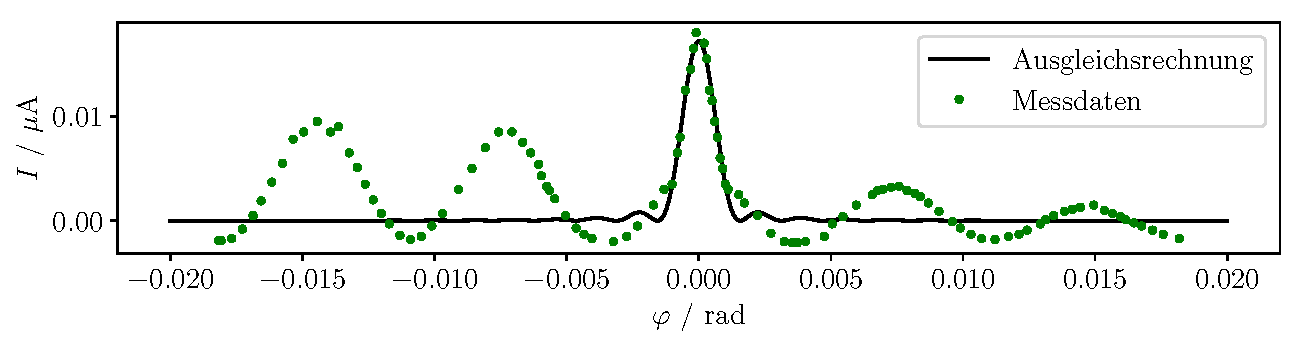
\includegraphics[height=5cm, width=15cm]{Auswertung/Graph_Einzelspalt1.pdf}
	\caption{Regression der Messwerte des ersten Einzelspaltes.}
	\label{fig:Einzel1}
\end{figure}
 
 Für die theoretisch bestimmte Spaltbreite $b$ ergibt sich somit:
 \begin{equation*}
 	b = 0.3240 \pm 0.0004
\end{equation*}
Die angegebene, tatsächliche Spaltbreite beträgt 0,1 mm. Somit ergibt sich eine Abweichung von 324\%.

Für den zweiten Einzelspalt wird analog vorgegangen. Die dazugehörigen Messwerte befinden sich in Tabelle $\mathbf{2}$.
\begin{table}
\label{tab:e2}
    \centering
\caption{Messwerte des Einzelspaltes (Breite 0.44mm).}
\begin{minipage}{0.46\textwidth}
    \centering
	\begin{tabular}{c|c|c}
		\toprule
		{$x / mm$} & {$I / A\cdot10^{-9}$} & {$I - I_\text{d} / A\cdot10^{-9}$}\\
		\hline
        \midrule
        0.0 &110.0&105.5\\
        0.1 &110.0&105.5\\
        0.2 &108.&103.5\\
        0.3 &105.0&100.5\\
        0.5 &100.0&95.5\\
        0.6 &90.0&85.5\\
        0.7 &85.0&80.5\\
        0.8 &80.0&75.5\\
        0.9 &75.0&70.5\\
        1.0 &70.0&65.5\\
        1.1 &65.0&60.5\\
        1.2 &60.0&55.5\\
        1.3 &60.0&55.5\\
        1.4 &54.0&49.5\\
        1.5 &50.0&45.5\\
        1.6 &46.0&41.5\\
        1.7 &44.0&39.5\\
        1.8 &40.0&35.5\\
        1.9 &37.0&32.5\\
        2.0 &34.0&29.5\\
        2.1 &30.0&25.5\\
        2.2 &28.0&23.5\\
        2.3 &25.0&20.5\\
        2.4 &24.0&19.5\\
        2.5 &22.0&17.5\\
        2.6 &21.0&16.5\\
        2.7 &20.0&15.5\\
        2.9 &21.0&16.5\\
        3.1 &23.0&18.5\\
        3.2 &24.0&19.5\\
		\bottomrule 
	\end{tabular}
\end{minipage}
\begin{minipage}{0.46\textwidth}
    \centering
	\begin{tabular}{c|c|c}
		\toprule
		{$x / mm$} & {$I / A\cdot10^{-9}$}& {$I - I_\text{d} / A\cdot10^{-9}$} \\
		\hline
        \midrule
        3.5 &20.0&15.5\\
        3.8 &26.0&21.5\\
        4.0 &26.0&21.5\\
        4.1 &25.0&20.5\\
        4.3 &24.0&19.5\\
        -0.1 &110.0&105.5\\
        -0.2 &110.0&105.5\\
        -0.3 &105.0&100.5\\
        -0.4 &100.0&95.5\\
        -0.7 &90.0&85.5\\
        -0.8 &80.0&75.5\\
        -1.0 &75.0&70.5\\
        -0.8 &80.0&75.5\\
        -1.0 &75.0&70.5\\
        -1.3 &65.0&60.5\\
        -1.5 &42.0&37.5\\
        -1.6 &38.0&33.5\\
        -1.8 &28.0&23.5\\
        -2.0 &24.0&19.5\\
        -2.2 &22.0&17.5\\
        -2.7 &24.0&19.5\\
        -2.9 &26.0&21.5\\
        -3.0 &26.0&21.5\\
        -3.2 &24.0&19.5\\
        -3.3 &22.0&17.5\\
        -3.4 &21.0&16.5\\
        -3.5 &20.0&15.5\\
        -3.8 &18.0&13.5\\
        -4.1 &17.0&12.5\\
        -4.3 &17.0&12.5\\
		\bottomrule 
	\end{tabular}
\end{minipage}
\end{table}

Die dazugehörige Regression ist in der Abbildung \ref{fig:b} abgebildet.

\begin{figure}[H]
    \centering
    \includegraphics{Auswertung/Graph2.pdf}
    \caption{Regression des zweiten Einzelspaltes.}
    \label{fig:b}
\end{figure}

 Für die theoretisch bestimmte Spaltbreite $b$ ergibt sich somit:
 \begin{equation*}
 	b = 0.325 \text{mm}
\end{equation*}
Die angegebene, tatsächliche Spaltbreite beträgt 0,44 mm. Somit ergibt sich eine Abweichung von 73,39\%.

\subsection{Messung der Beugung am Doppelspalt}

Die Messdaten der Messung am Doppelspalt sind in Tabelle $\mathbf{3}$ zu finden. $x$ ist dabei der Abstand von der Mitte des Verschiebereiters der Photodiode, an dem gemessen wird. $I$ ist der gemessene Strom des Amperemeters.

\begin{table}
\label{tab:Tabelle1}
	\centering
\caption{Messwerte des Doppelspaltes.}
\begin{minipage}{0.46\textwidth}
    \centering
	\begin{tabular}{c|c|c}
		\toprule
		{$x / mm$} & {$I / A\cdot10^{-9}$}& {$I - I_\text{d} / A\cdot10^{-9}$} \\
		\hline
        \midrule
        0.0 &23.0&18.5\\
        0.2 &22.0&17.5 \\
        0.4 &20.0&15.5\\
        0.5 &18.0 &13.5\\
        0.6 &17.5&13.0\\
        0.7 &17.0&12.5\\
        0.8 &17.5&13.0\\
        0.9 &18.0&13.5\\
        1.0 &19.0&14.5\\
        1.2 &22.0&17.5\\
        1.4 &22.0&17.5\\
        1.5 &21.0&16.5\\
        1.6 &19.0&14.5\\
        1.7 &17.5&13.0\\
        1.9 &15.0&10.5\\
        2.1 &16.0&11.5\\
        2.3 &19.0&14.5\\
        2.4 &20.0&15.5\\
        2.5 &20.5&16.0\\
        2.7 &18.0&13.5\\
        2.9 &15.0&10.5\\
        3.0 &13.0&8.5\\
        3.1 &12.0&7.5\\
        3.4 &13.0&8.5\\
        3.5 &15.0&10.5\\
        3.6 &16.0&11.5\\
        3.7 &17.5&13.0\\
        3.9 &17.5&13.0\\
        4.0 &16.0&11.5\\
        4.1 &13.0&8.5\\
        4.2 &12.0&7.5\\
        4.3 &11.0&6.5\\
        4.4 &9.5&5.0\\
		\bottomrule 
	\end{tabular}
\end{minipage}
\begin{minipage}{0.46\textwidth}
    \centering
	\begin{tabular}{c|c|c}
		\toprule
		{$x / mm$} & {$I / A\cdot10^{-9}$}& {$I - I_\text{d} / A\cdot10^{-9}$} \\
		\hline
        \midrule
        4.7 &10.0&5.5\\
        4.8 &11.0&6.5\\
        4.9 &13.0&8.5\\
        5.0 &14.5&10.0\\
        5.3 &13.0&8.5\\
        5.4 &12.0&7.5\\
        5.5 &10.0&5.5\\
        5.6 &8.0&3.5\\
        5.7 &7.5&3.0\\
        5.9 &8.0&3.5\\
        6.0 &9.0&4.5\\
        6.2 &12.0&7.5\\
        6.4 &12.5&8.0\\
        6.5 &12.0&7.5\\
        6.6 &11.0&6.5\\
        6.7 &9.0&4.5\\
        6.8 &8.0&3.5\\
        6.9 &7.0&2.5\\
        7.0 &6.5&2.0\\
        7.2 &8.0&3.5\\
        7.4 &10.0&5.5\\
        7.6 &9.0&4.5\\
        7.7 &8.0&3.5\\
        7.8 &7.0&2.5\\
        7.9 &6.5&2.0\\
        8.0 &6.0&1.5\\
        8.2 &7.5&3.0\\
        8.4 &8.0&3.5\\
        8.6 &8.0&3.5\\
        8.8 &7.5&3.0\\
        9.0 &7.0&2.5\\
        9.2 &6.5&2.0\\
        9.5 &7.5&3.0\\
		\bottomrule 
	\end{tabular}
\end{minipage}
\end{table}
\begin{table}
\centering
\begin{minipage}{0.46\textwidth}
    \centering
	\begin{tabular}{c|c|c}
		\toprule
		{$x / mm$} & {$I / A\cdot10^{-9}$} & {$I - I_\text{d} / A\cdot10^{-9}$}\\
		\hline
        \midrule
        9.8 &7.5&3.0\\
        10.3 &7.0&2.5\\
        10.6 &6.5&2.0\\
        10.7 &6.0&1.5\\
        11.0 &7.0&2.5\\
        11.5 &7.0&2.5\\
        12.0 &5.5&1.0\\
        12.3 &6.0&1.5\\
        12.5 &6.5&2.0\\
        12.6 &7.0&2.5\\
        12.7 &6.5&2.0\\
        12.8 &6.6&2.1\\
        12.9 &6.2&1.7\\
        13.0 &5.8&1.3\\
        13.1 &5.6&1.1\\
        13.4 &5.8&1.3\\
        13.5 &6.1&1.6\\
        13.6 &6.4&1.9\\
        13.7 &6.6&2.1\\
        13.8 &6.7&2.2\\
        13.9 &6.5&2.0\\
        14.0 &6.0&1.5\\
        14.1 &5.7&1.2\\
        14.2 &5.4&0.9\\
        14.3 &5.2&0.7\\
        14.5 &5.5&1.0\\
        14.6 &5.7&1.2\\
        14.8 &5.9&1.4\\
        15.0 &6.0&1.5\\
        15.2 &5.7&1.2\\
        15.3 &5.4&0.9\\
        15.4 &5.2&0.7\\
        15.5 &5.0&0.5\\
		\bottomrule 
	\end{tabular}
\end{minipage}
\begin{minipage}{0.46\textwidth}
    \centering
	\begin{tabular}{c|c|c}
		\toprule
		{$x / mm$} & {$I / A\cdot10^{-9}$} & {$I - I_\text{d} / A\cdot10^{-9}$}\\
		\hline
        \midrule
        -0.0 &23.0&18.5\\
        -0.2 &22.0&17.5\\
        -0.4 &20.0&15.5\\
        -0.5 &20.0&15.5\\
        -0.6 &19.0&14.5\\
        -0.7 &18.5&14.0\\
        -0.8 &19.0&14.5\\
        -0.9 &20.0&15.5\\
        -1.0 &21.0&16.5\\
        -1.2 &22.0&17.5\\
        -1.4 &21.5&17.0\\
        -1.5 &21.0&16.5\\
        -1.6 &21.0&16.5\\
        -1.7 &20.0&15.5\\
        -1.9 &18.0&13.5\\
        -2.1 &19.0&14.5\\
        -2.3 &20.0&15.5\\
        -2.4 &20.5&16.0\\
        -2.5 &20.0&15.5\\
        -2.7 &19.0&14.5\\
        -2.9 &18.0&13.5\\
        -3.0 &17.5&13.0\\
        -3.1 &17.5&13.0\\
        -3.4 &18.0&13.5\\
        -3.5 &18.5&14.0\\
        -3.6 &18.0&13.5\\
        -3.7 &17.5&13.0\\
        -3.9 &16.0&11.5\\
        -4.0 &15.0&10.5\\
        -4.1 &14.5&10.0\\
        -4.2 &14.0&9.5\\
        -4.3 &14.4&9.9\\
        -4.4 &15.0&10.5\\
		\bottomrule 
	\end{tabular}
\end{minipage}
\end{table}
\begin{table}
\centering
\begin{minipage}{0.46\textwidth}
    \centering
	\begin{tabular}{c|c|c}
		\toprule
		{$x / mm$} & {$I / A\cdot10^{-9}$} & {$I - I_\text{d} / A\cdot10^{-9}$} \\
		\hline
        \midrule
        -4.7 &15.5&11.0\\
        -4.8 &15.5&11.0\\
        -4.9 &15.0&10.5\\
        -5.0 &14.5&10.0\\
        -5.3 &12.5&8.0\\
        -5.4 &12.0&7.5\\
        -5.5 &11.0&6.5\\
        -5.6 &11.0&6.5\\
        -5.7 &11.5&7.0\\
        -5.9 &12.0&7.5\\
        -6.0 &12.5&8.0\\
        -6.2 &12.0&7.5\\
        -6.4 &11.0&6.5\\
        -6.5 &10.0&5.5\\
        -6.6 &9.4&4.9\\
        -6.7 &8.6&4.1\\
        -6.8 &8.4&3.9\\
        -6.9 &8.5&4.0\\
        -7.0 &8.7&4.2\\
        -7.2 &9.5&5.0\\
        -7.4 &9.8&5.3\\
        -7.6 &9.4&4.9\\
        -7.7 &8.7&4.2\\
        -7.8 &8.1&3.6\\
        -7.9 &7.4&2.9\\
        -8.0 &7.0&2.5\\
        -8.2 &6.8&2.3\\
        -8.4 &7.4&2.9\\
        -8.6 &8.0&3.5\\
        -8.8 &8.2&3.7\\
        -9.0 &7.5&3.0\\
        -9.2 &6.6&2.1\\
        -9.5 &6.2&1.7\\
		\bottomrule 
	\end{tabular}
\end{minipage}
\begin{minipage}{0.46\textwidth}
    \centering
	\begin{tabular}{c|c|c}
		\toprule
		{$x / mm$} & {$I / A\cdot10^{-9}$}& {$I - I_\text{d} / A\cdot10^{-9}$} \\
		\hline
        \midrule
        -9.8 &7.1&2.6\\
        -10.3 &7.0&2.5\\
        -10.6 &6.2&1.7\\
        -10.7 &6.2&1.7\\
        -11.0 &6.9&2.4\\
        -11.5 &7.2&2.7\\
        -12.0 &6.2&1.7\\
        -12.3 &7.0&2.5\\
        -12.5 &7.4&2.9\\
        -12.6 &7.4&2.9\\
        -12.7 &7.1&2.6\\
        -12.8 &6.8&2.3\\
        -12.9 &6.5&2.0\\
        -13.0 &6.2&1.7\\
        -13.1 &6.1&1.6\\
        -13.4 &6.4&1.9\\
        -13.5 &6.6&2.1\\
        -13.6 &6.9&2.4\\
        -13.7 &7.0&2.5\\
        -13.8 &6.9&2.4\\
        -13.9 &6.7&2.2\\
        -14.0 &6.4&1.9\\
        -14.1 &6.2&1.7\\
        -14.2 &5.9&1.4\\
        -14.3 &5.8&1.3\\
        -14.5 &5.8&1.3\\
        -14.6 &5.8&1.3\\
        -14.8 &6.2&1.7\\
        -15.0 &6.3&1.8\\
        -15.2 &6.1&1.6\\
        -15.3 &6.0&1.5\\
        -15.4 &5.8&1.3\\
        -15.5 &5.6&1.1\\
		\bottomrule 
	\end{tabular}
\end{minipage}
\end{table}

Die Spaltgröße $b$ und Gitterkonstante $s$ werden beim Doppelspalt analog zu den obigen Einzelspalten bestimmt, jedoch anhand der Gleichung \ref{eqn:IntDop}. Die Regression ist in Abbildung \ref{fig:Doppel} dargestellt.

 \begin{figure}[h]
	\centering
	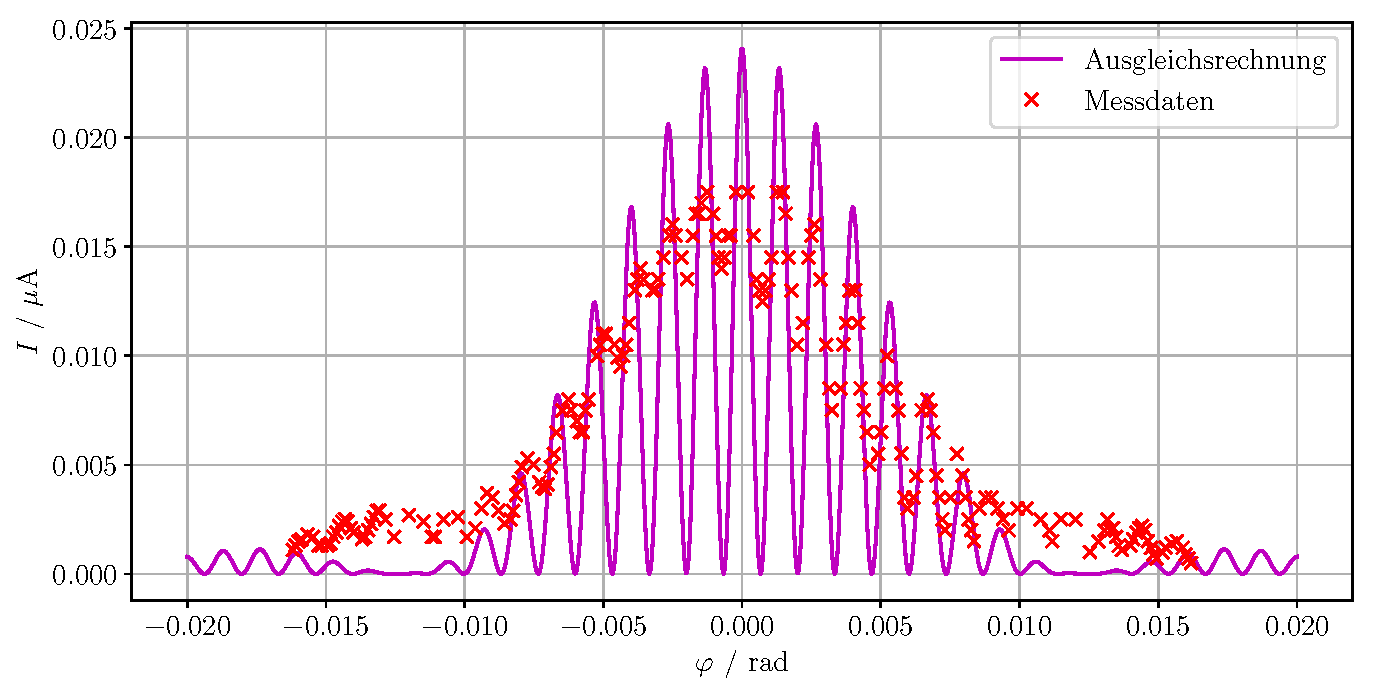
\includegraphics[height=10cm, width=15cm]{Auswertung/Graph_doppel.pdf}
	\caption{Regression der Messwerte des Doppelspaltes.}
	\label{fig:Doppel}
\end{figure}
 
 Für die theoretisch bestimmte Spaltbreite $b$ und Gitterkonstante $s$ ergeben sich somit:
 \begin{gather*}
 	b =  1.6508 \pm 1.904\cdot10^{-4} \text{mm}\\
	s = 1.5108 \pm 4.736\cdot10^{-4} \text{mm}
\end{gather*}
Die angegebene, tatsächliche Spaltbreite beträgt 0,1 mm. Somit ergibt sich eine Abweichung von 1650\%.
Die angegebene, tatsächliche Gitterkonstante beträgt 0,1 mm. Somit ergibt sich eine Abweichung von 1510\%.

In der folgenden Abbildung \ref{fig:Vergleich} ist ein Vergleich des Einzelspaltes mit Spaltbreite und dem Doppelspalt zu sehen:

 \begin{figure}[h]
	\centering
	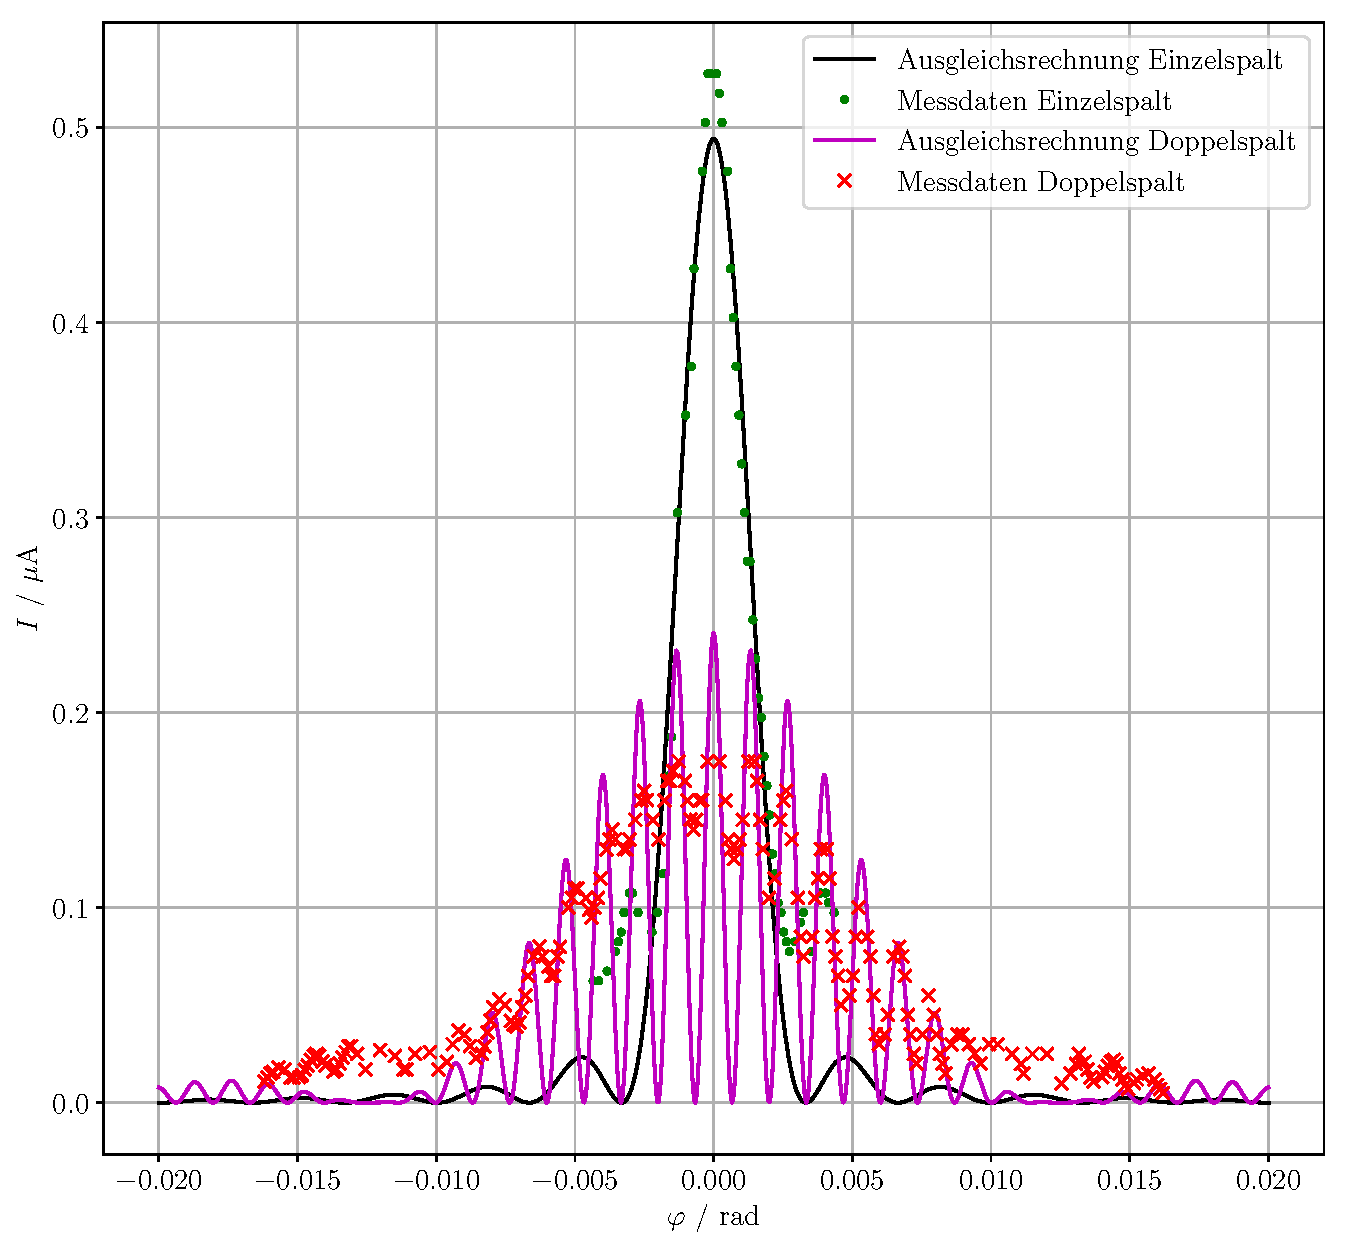
\includegraphics[height=11cm, width=15cm]{Auswertung/Vergleich.pdf}
	\caption{Vergleich des Einzelspaltes mit dem Doppelspalt.}
	\label{fig:Vergleich}
\end{figure}
